\documentclass[12pt,twoside,a4]{article}
\usepackage{amsmath}
\usepackage{amssymb}
\usepackage{amsfonts}
\usepackage{array}
\usepackage{graphicx}% use this package if an eps figure is included.
\usepackage{wrapfig}
\usepackage{mathrsfs}
\usepackage{multirow}
\usepackage{enumitem}
\newlist{steps}{enumerate}{1}
\setlist[steps, 1]{label = Step \arabic*:}
\usepackage[version=4]{mhchem}
\setlength\topmargin{-1.1in} \addtolength\textheight{2.1in}
\addtolength{\oddsidemargin}{-0.5in} \textwidth 6.5in
\addtolength{\evensidemargin}{-1in} \textwidth 6.5in
\newcounter{questioncounter}
\newcounter{equestioncounter}
\setlength\parskip{10pt} \setlength\parindent{0in}
\newcommand{\bea}{\begin{eqnarray*}}
\newcommand{\eea}{\end{eqnarray*}}
\newcommand{\beao}{\begin{eqnarray}}
\newcommand{\eeao}{\end{eqnarray}}
\newcommand{\no}{\noindent}
\begin{document}
\title{Cleaning Dirty Pennies}
\date{Friday, February 2, 2018}
\author{By: Katelyn Talbot\\
\small Mrs. Ruffalo's Kindergarten Class}
\maketitle
\section{Abstract}
In this experiment we will attempt to clean old pennies (ones that look dirty) with a solution of vinegar and salt.

\section{Introduction}
The outside of a penny is made of copper.  Copper is a metal which has a reddish brown or orange color.  Over time as copper is exposed to air and other substances in the air, the copper will change in color. It may turn black, brown, bluish-green or green depending on the environment the penny is exposed too.  For example, today the Statue of Liberty is green in color, but over a hundred years ago she was a dull copper color like a penny.  After years of exposure to ocean air her copper skin turned the iconic green color it is today.
\begin{wrapfigure}{htb}{0.3\textwidth}
\centering
% Requires \usepackage{graphicx}
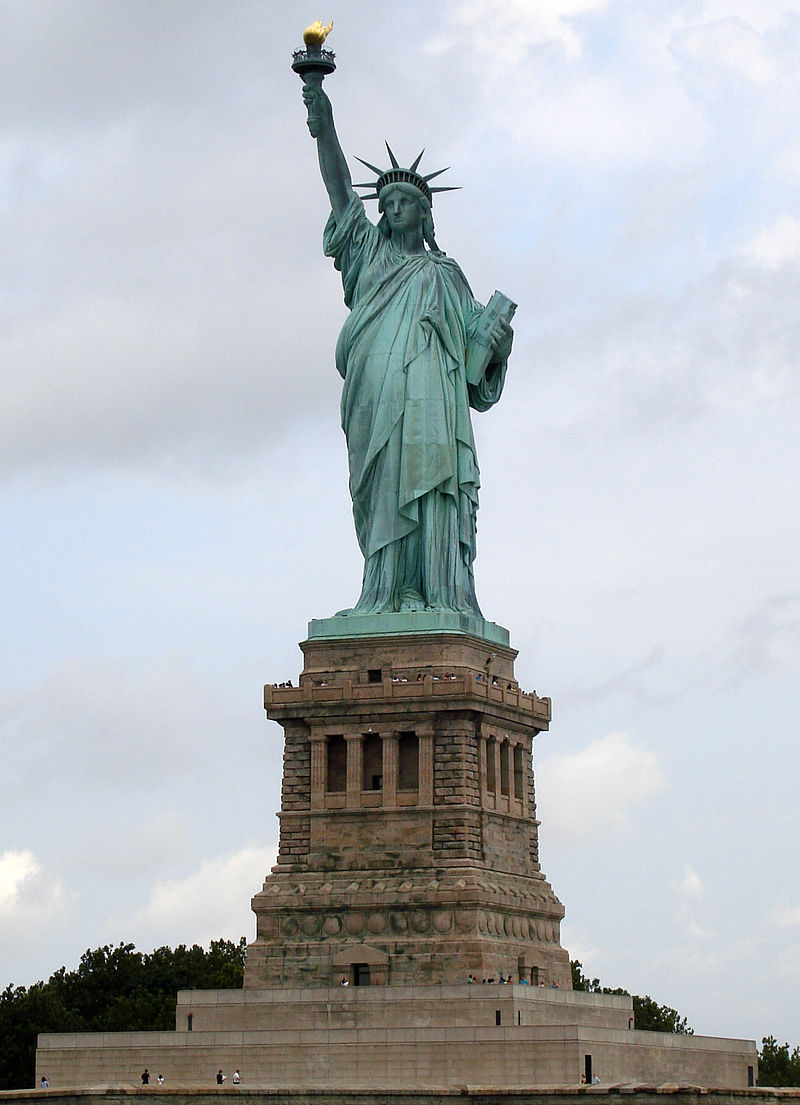
\includegraphics[width=0.25\textwidth]{Statue_of_Liberty.jpg}
\caption{Statue of Liberty.}\label{sol}
\end{wrapfigure}
%\flush

Today's experiment will focus on one way a to clean old pennies using two simple substances found in almost any kitchen:
\begin{enumerate}[noitemsep]
\item Acetic Acid, aka \textbf{Vinegar} (chemical formula: \ce{CH3COOH}),
\item Sodium Cloride, aka \textbf{Salt} (chemical formula: \ce{NaCl})
\end{enumerate}

%\begin{figure}[h]
%\begin{center}
%  % Requires \usepackage{graphicx}
%  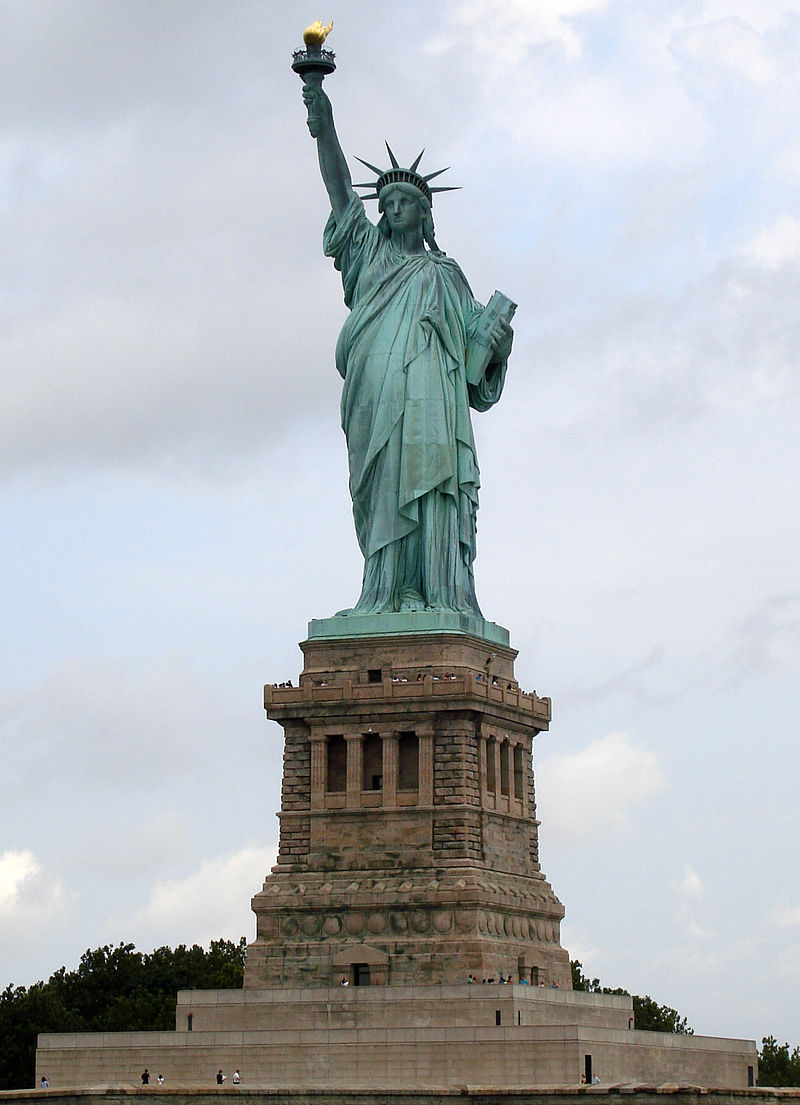
\includegraphics[width=0.25\textwidth]{Statue_of_Liberty.jpg}\\
%  \caption{Statue of Liberty.}\label{sol}
%  \end{center}
%\end{figure}
To be sure we can see a change we need to have a control.  The control will be used to compare an untested sample against a sample that has under gone the experiment.  Finding two pennies that are identical in color and age will be hard.  So for this experiment we will test only half the penny, the other half of the penny will not be dipped into the solution.  This will allow one half to be the control and the other half will be the test.

\section{Needed Supplies}
\begin{itemize}%[noitemsep]
\item Glass or Ceramic bowl,
\item old Pennies darkened from age,
\item vinegar,
\item table salt and
\item a spoon for mixing.
\end{itemize}

\section{Procedure}
For this experiment we will follow the steps below:
\begin{steps}
\setlength\itemindent{25pt}
\item Pour about one tablespoon of vinegar into a glass or ceramic dish.
\item Add about one teaspoon of salt.
\item Mix vinegar and salt for 1 minute.
\item Dip only half or less of the penny into the solution and count to 10.
\item Remove penny and rinse in cold water.
\item Look for any differences between the penny halves.  Is one side a different color than the other?  You can also try dipping it in again for another 10 seconds to see what happens.
\end{steps}

This experiment will clean a penny if the penny was indeed dirty because of oxidation, exposure to air over time.  Pennies spend a lot of time in people's pockets and can get dirty from things that this acidic solution will not clean away.  So if you don't see any change, try another penny in case the dirt on your penny is not due to something other than oxidation.

\section{Why does this happen..}

Oxidization only forms on the outer layer of the copper penny (the portion which is exposed to air).  When the oxidized penny is dipped into the salt and vinegar solution the outer layer of oxidized copper under goes a chemical reaction which dissolves the oxidation.  This reaction exposes the natural color of the copper metal underneath the dark oxidation layer.  Unoxidized copper will not react with the acidic solution so the reaction stops leaving a clean penny.



\end{document} 